\documentclass{article}

\textwidth=6.5in
\textheight=8.5in
\voffset=-54pt
\oddsidemargin=0in
\evensidemargin=0in
\setlength{\parskip}{8pt}
\setlength{\parindent}{0pt}

\usepackage{amsmath, amssymb}
\usepackage{ifthen}

\usepackage[inline]{enumitem}
\setlist{topsep=0pt, parsep=8pt}

\usepackage[rgb,table]{xcolor}\convertcolorsUfalse
\usepackage{graphicx}

% change hyperref options
\PassOptionsToPackage{hyphens}{url}
\usepackage[bookmarks,colorlinks,linkcolor=black,citecolor=blue,pdfstartview=FitH,urlcolor=blue]{hyperref}
\hypersetup{pdfpagemode=UseNone}
\usepackage{bookmark}

\usepackage{graphicx}
\usepackage{multicol}
\usepackage{framed}
\usepackage{array}

\usepackage{icomma}

\usepackage{marginnote}
\usepackage[colorinlistoftodos]{todonotes}
\renewcommand{\marginpar}{\marginnote}

\usepackage{soul}

\usepackage{tikz}
\usetikzlibrary{
  matrix,%
  % enables the snake paths
  decorations.pathmorphing,%
  % enables bigger arrows
  decorations.markings,%
  decorations.pathreplacing,%
  decorations.text,%
  calc,%
  patterns,%
  shapes.geometric,%
  arrows,
  decorations.shapes,
  positioning,
  plotmarks,
  intersections
}
\tikzset{>=latex} % sets default arrow type in tikz
\tikzset{font=\normalsize}
\tikzset{mark size=1.5pt, mark options=thin}
\tikzset{pin distance=4pt,
  every pin edge/.style={<-, thin, shorten <= -2pt}}

\interfootnotelinepenalty=10000
\renewcommand{\thefootnote}{(\arabic{footnote})}

\usepackage{multirow, bigdelim}

% change to \usepackage[sols]{handout} to see solutions
\usepackage[]{handout}

\newcommand\iscurrentenumi[1]{%
  \ifthenelse{\equal{#1}{\theenumi}}{}{#1}}
\setenumerate[1]{ref=\#\arabic*}
\setenumerate[2]{ref=\protect\iscurrentenumi{\theenumi}(\alph*)}
\newcommand\enumiiprefix[2]{%
  \ifthenelse{{\equal{#1}{\theenumi}}\AND{\equal{#2}{(\alph{enumii})}}}{}{}%
  \ifthenelse{{\equal{#1}{\theenumi}}\AND{\NOT{\equal{#2}{(\alph{enumii})}}}}{#2}{}%
  \ifthenelse{\equal{#1}{\theenumi}}{}{#1#2}%
}
\setenumerate[3]{ref=\protect\enumiiprefix{\theenumi}{(\alph{enumii})}\roman*}

\newlength{\tipmargin}
\makeatletter

\newdimen\SOUL@dimen %new
\def\SOUL@ulunderline#1{{%
    \setbox\z@\hbox{#1}%
    % \dimen@=\wd\z@
    \SOUL@dimen=\wd\z@ %new
    \dimen@i=\SOUL@uloverlap
    \advance\SOUL@dimen2\dimen@i %\dimen@ exchanged too
    \rlap{%
      \null
      \kern-\dimen@i
      % \SOUL@ulcolor{\SOUL@ulleaders\hskip\dimen@}%
      \SOUL@ulcolor{\SOUL@ulleaders\hskip\SOUL@dimen}% new
    }%
    \unhcopy\z@
  }}

\renewenvironment{framed}{
  \setlength{\tipmargin}{\textwidth-\linewidth}
  \advance\@totalleftmargin-\tipmargin
  \def\FrameCommand{\hspace{\tipmargin}\fbox}%
  \advance\linewidth\tipmargin
  \MakeFramed {\advance\hsize-\width \FrameRestore}%
}
{\endMakeFramed}

\makeatother

\definecolor{purple}{rgb}{0.5,0,1.0}
\definecolor{hotpink}{rgb}{1, 0, 0.5}

\definecolor{skyblue}{rgb}{0, 0.5, 1}

\newcommand{\goal}[1]{\textbf{\textcolor{skyblue}{#1}}}
\newcommand{\indvar}[1]{\textbf{\textcolor{hotpink}{#1}}}

\usepackage{fancyhdr}
\lhead{\textcolor{white}{This content is protected and may not be shared, uploaded, or distributed.}}
\rhead{}
\rfoot{\vspace*{\fill}\footnotesize\textcopyright{} \emph{Harvard Math Ma}}
\renewcommand{\headrulewidth}{0pt}
\pagestyle{fancy}
\begin{document}

\htitle{Function Composition, Modeling with Functions}

\begin{problemonly}
  \begin{framed}

You should be able to:
    \begin{itemize}[topsep=0pt,partopsep=0pt,parsep=8pt,itemsep=0pt]
    \item Explain how composition of functions models situations where there is a chain of dependency among variables.

    \item Compute compositions of functions.

    \item Model situations systematically: identify your goal, define variables and express your goal in terms of those variables, and then look for relationships among your variables.

    \item Communicate your modeling process clearly. 
    \end{itemize}
  \end{framed}
\end{problemonly}

\begin{enumerate}
\item 

  \note{This is a situation where composition arises naturally, so I'll just let them try it and then let them know that this is called function composition.} 

  The price of tomatoes varies seasonally; suppose $P(x)$ gives the price of tomatoes in dollars per pound at time $x$. The demand for tomatoes (in other words, the amount of tomatoes people want to buy) depends on the price; say that $D(x)$ gives the demand for tomatoes when they cost \$$x$ per pound.

  Answer the following questions using functional notation. 

  \begin{enumerate}
  \item
    \begin{problem}[\vfill]
      When tomatoes cost \$3 per pound, what is the demand for tomatoes? 
    \end{problem}

    \begin{solution} 
      $D(3)$
    \end{solution}

  \item
    \begin{problem}[\vfill] 
      At time $3$, what is the demand for tomatoes? 
    \end{problem}

    \begin{solution} 
      $D(P(3))$
    \end{solution}

  \item
    \begin{problem}[\vfill]
      What's the demand for tomatoes at time $t$? 
    \end{problem}

    \begin{solution}
      $D(P(t))$
    \end{solution}

  \end{enumerate} 

\item 

  \emph{Working algebraically with compositions}. If $f(x) = x^2$ and $h(x) = 2x-1$, find each of the following.

  \begin{enumerate}

  \item

    \note{I might also ask students whether $(2x - 1)^2$ is the same as $2x - 1^2$.}

    \begin{problem}[\vfill]
      $f(h(x))$
    \end{problem}

    \begin{solution}
      Since $h(x) = 2x - 1$, this is the same as $f(2x - 1)$, or $\boxed{(2x - 1)^2}$.
    \end{solution}

  \item
    \begin{problem}[\vfill\newpage]
      $h(f(x))$
    \end{problem}

    \begin{solution}
      Since $f(x) = x^2$, this is the same as $h(x^2) = \boxed{2x^2 - 1}$.
    \end{solution}

  \end{enumerate}

\item  \label{modeling-rectangular-pen-1}

  \begin{enumerate}
  \item
    \begin{problem}[\vfill]
      Harvard's Hollis Professor of Divinity (currently Karen King) has the right to graze animals in Harvard Yard.\footnote{\url{https://news.harvard.edu/gazette/story/2012/05/the-oldest-endowed-professorship/}} Professor King wants to have some room for her cow to roam in without escaping, so she decides to build a rectangular fenced-in pen using 28 feet of wire fencing. She'd like to understand how much area the pen could have, so she asks you to model the area of the pen as a function of the length of one side. Help her out! (Assume that she will use all 28 feet of fencing.)
    \end{problem}

    \begin{solution}
      Here's a general strategy for problems like this.
      \begin{enumerate}[label=\arabic*.]
      \item \hl{\textbf{Understand the Problem.}}

        \begin{itemize}
        \item \hl{\textbf{Goal:}} Express the \goal{area} of the pen as a function of the \indvar{length of one side}.

          \hl{\textbf{Know:}} perimeter = 28 feet

        \item Drawing \textbf{a couple of examples} is a great way to get a feel for the situation; I try to make my examples very different from each other. Here are two examples of pens with perimeter 28 feet:
          \begin{center}
            \begin{tikzpicture}[scale = .2]
              \draw (0, 0) -| (7, 7) node[pos=0.25, below] {$7$ feet} node[pos=0.75, right] {$7$ feet} -| (0, 0); %
              \draw (20, 2.5) -| (32, 4.5) node[pos=0.25, below] {$12$ feet} node[pos=0.75, right] {$2$ feet} -| (20, 2.5); %
            \end{tikzpicture}
          \end{center}
        \end{itemize}

      \item Since our goal is the \goal{area}, let's \hl{\textbf{write a formula}} for it, \hl{\textbf{defining any variables we use}} (either in words or by labeling them in a picture). At this stage, it's okay if the formula involves more than one variable.

        \begin{center}
          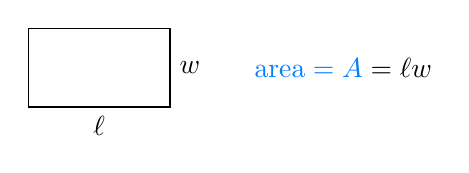
\begin{tikzpicture}[scale = .2]
            \draw (0, 0) -| (9, 5) node[pos=0.25, below] {$\ell$ } node[pos=0.75, right] {$w$ } -| (0, 0); \draw (20, 2.5) node{$\color{skyblue}{\text{area}} = A\color{black} = \ell w$};
          \end{tikzpicture}
        \end{center}

      \item Now, we need to \hl{\textbf{relate the variables we've used}} so that we can get everything in terms of the desired variable, \indvar{length of one side ($\ell$)}.\footnote{You could also express it in terms of $w$, since $w$ is also the length of one side.} To do this, we must \hl{\textbf{use something we know about the situation}}. Here, the thing we know is that the perimeter is 28 feet, so
        \begin{align*}
          2w + 2 \ell &= 28 \\
          \intertext{Using this equation, we can now express $w$ in terms of the desired variable \indvar{$\ell$}:}
          2w &= 28 - 2 \ell \\
          w &= 14 - \ell
        \end{align*}
        Plugging this back into our area formula, $A = \ell w = \boxed{\ell (14 - \ell)}$.

      \end{enumerate}
    \end{solution}

  \item
    \begin{problem}[1in]
      What's the domain of the function in (a)? 
    \end{problem}

    \begin{solution}
      The domain is the set of all possible input values, so all of the possible values for $\ell$. No restrictions are explicitly stated in the problem, but we could reasonably
      argue that both $\ell$ and $w$ should be non-negative, $\ell \geq 0$ and $w \geq 0$. 
      (You could also reasonably argue that $\ell$ and $w$ should be strictly positive, and that would be fine as well
      in this case.)
      
      Since $\ell \geq 0$, this gives us a minimum possible value of $\ell$. 
      The restriction $w \geq 0$ means that we will
      have a maximum possible value of $\ell$, since the perimeter is 28 feet. We can find the maximum possible
      value by solving an inequality.
      \begin{align*}
          w & \geq 0 \\
          14- \ell & \geq 0 \\
          - \ell & \geq -14 \\
          \ell & \leq 14
      \end{align*}
      So the domain is $\boxed{0 \leq \ell \leq 14}$.
    \end{solution}

  \end{enumerate}

  \pspace{\newpage}



\item  % Based on Otto Bretscher's Lecture Notes on Calculus, 8.1.6

  Your snowmobile runs out of gas when you're 3 miles south of a major highway. The nearest gas station is on the highway 6 miles east of your position. You decide to head for some point on the highway and then walk along the highway until you reach the gas station, as shown in the diagram.

  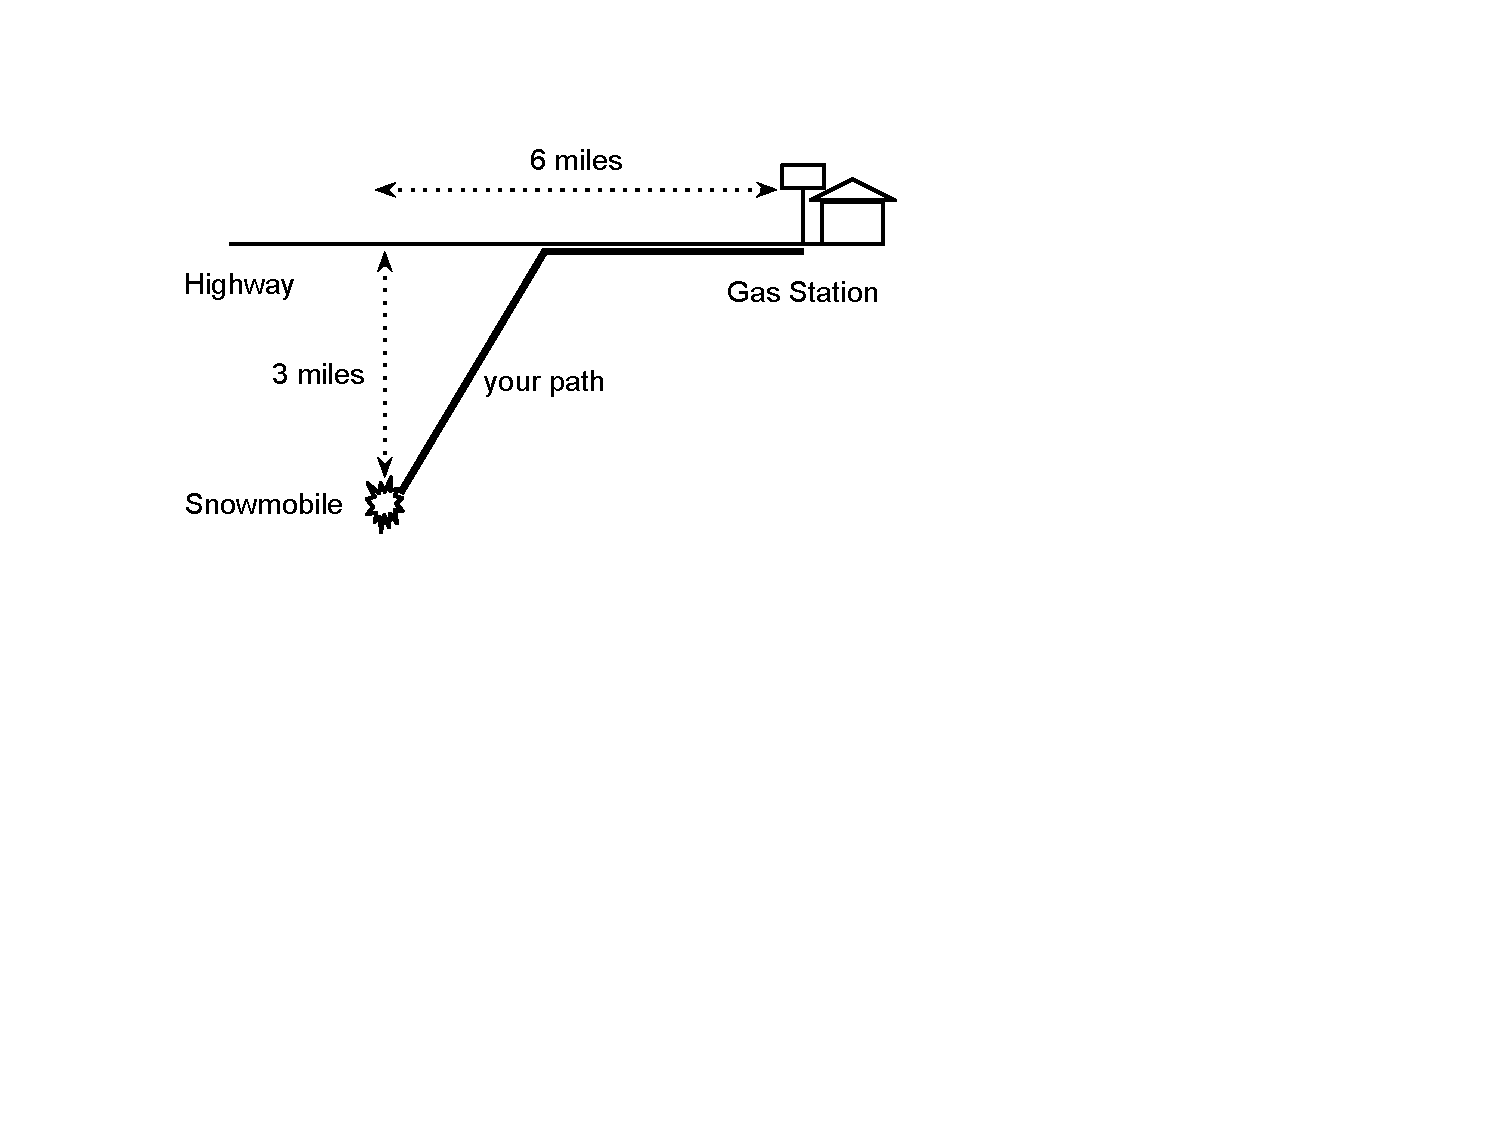
\includegraphics[width = 3in]{images/snowmobile.pdf}

  \begin{enumerate}
  \item
    \begin{problem}[\vfill]
      If you choose a path that involves walking $h$ miles along the
      highway, how many miles will you walk through the snow? (Express
      your answer in terms of $h$.) 
    \end{problem}

    \begin{solution}
      \hl{\textbf{Our goal}} is to write the \goal{total distance} we walk to get to the gas station
      in terms of the \indvar{distance along the highway}
      that we walk. \hl{\textbf{We know}} that we are 3 miles south and 6 miles west of the gas station.

      We can \hl{\textbf{draw pictures}} of different paths that we might take.
      \begin{center}
      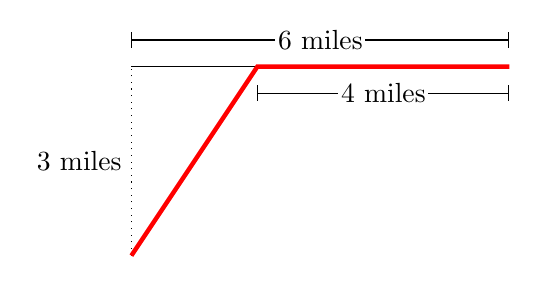
\begin{tikzpicture}[scale=0.8]
        \draw[dotted] (0,0) -- node[midway, left] {3 miles} (0,3);
        \draw (0,3) -- (6,3);
        \draw[|-|, yshift=12pt] (0,3) -- node[midway, inner sep=1pt, fill=white] {6 miles} (6,3);
        \draw[ultra thick, red] (0,0) -- (2, 3) -- (6, 3);
        \draw[|-|, yshift=-12pt] (2,3) -- node[midway, inner sep=1pt, fill=white] {4 miles} (6,3);
      \end{tikzpicture} \hspace{12pt}
      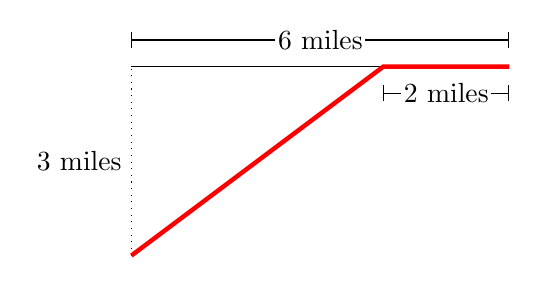
\begin{tikzpicture}[scale=0.8]
        \draw[dotted] (0,0) -- node[midway, left] {3 miles} (0,3);
        \draw (0,3) -- (6,3);
        \draw[|-|, yshift=12pt] (0,3) -- node[midway, inner sep=1pt, fill=white] {6 miles} (6,3);
        \draw[ultra thick, red] (0,0) -- (4, 3) -- (6, 3);
        \draw[|-|, yshift=-12pt] (4,3) -- node[midway, inner sep=1pt, fill=white] {2 miles} (6,3);
      \end{tikzpicture}
      \end{center}

      Now we can \hl{\textbf{write a formula}} for the total distance and \hl{\textbf{define any variables we use}}.
      \begin{center}
      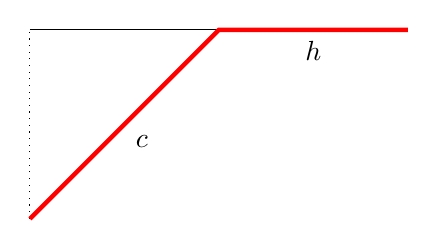
\begin{tikzpicture}[scale=0.8]
        \draw[dotted] (0,0) -- (0,3);
        \draw (0,3) -- (6,3);
        \draw[ultra thick, red] (0,0) -- node[midway, below right, black] {$c$} (3, 3) -- 
        node[midway, below, black] {$h$} (6, 3);
      \end{tikzpicture}
      \end{center}
      We're told in the problem to use $h$ for the distance we walk along the highway. If we call the total distance $d$,
      then $d=h+c$, where $c$ is diagonal distance that we walk through the snow.

      Now, to write $d$ as a function of $h$, we need to \hl{\textbf{relate the variables}} we used
      by \hl{\textbf{using information we know about the situation}} to replace
      $c$ with an equivalent expression in terms of $h$. Looking at the pictures we drew, we can see that $c$ is the
      hypotenuse of a right triangle, and we can express the lengths of the legs of the right triangle in terms of $h$.
      \begin{center}
      \begin{tikzpicture}[scale=0.8]
        \draw (0,0) -- node[midway, left] {$3$} (0,3);
        \draw (0,3) -- node[midway, above] {$6-h$} (4,3);
        \draw (0,0) -- node[midway, below right, black] {$c$} (4, 3);
      \end{tikzpicture}
      \end{center}
      We can use the Pythagorean theorem to say that $(3-h)^2+3^2=c^2$, and we can solve this for
      $c$ to get
      $c=\sqrt{(6-h)^2+3^2}$. Substituting for $c$ in $d=h+c$, we obtain
      $d=\boxed{h+\sqrt{(6-h)^2+3^2}}$.
    \end{solution}

  \item
    \begin{problem}[\vfill\newpage]
      You can walk 3 miles per hour on roads but only 2 miles per hour through snowy fields.

      If you choose a path that involves walking $h$ miles along the highway, how long will it take you to reach the gas station? (Again, express your answer in terms of $h$.)
    \end{problem}

    \begin{solution}
      This is similar to part (a), but now \hl{\textbf{our goal}} is to write down the \goal{total time} 
      it takes for us to walk to the gas station in terms of the \indvar{distance along the highway} that we walk.
      
      Referring to our pictures from above, we can \hl{\textbf{write a formula}} for the total time,
      \hl{\textbf{defining any variables we use.}} First, we can say that $\Delta t_\text{total} = 
      \Delta t_1 + \Delta t_2$, where
      $\Delta t_\text{total}$ is the total time, $\Delta t_1$ is the time spent walking the diagonal path through the snow, and
      $\Delta t_2$ is the time spent walking along the highway. 

      To write $\Delta t_\text{total}$ as a function of $h$, we need to \hl{\textbf{relate the variables}} we used to
      $h$. When traveling at a constant speed, $\text{distance} = \text{speed} \times \text{time}$. Since we can walk
      3 miles per hour on roads, we can write $h = 3 \Delta t_2$, so $\Delta t_2 = \frac{1}{3}h$. Since we can
      walk 2 miles per hours through the snow, we can write $c = 2 \Delta t_1$, so $\Delta t_1 = \frac{1}{2}c$, where
      $c$ is the diagonal distance we defined from before. We found in part (a) that $c=\sqrt{(6-h)^2+3^2}$, and
      substituting this for $c$ gives us $\Delta t_1 = \frac{1}{2}\sqrt{(6-h)^2+3^2}$.

      Putting everything together, we find that $\Delta t_\text{total} = 
      \boxed{\frac{1}{2}\sqrt{(6-h)^2+3^2} + \frac{1}{3}h}$.
    \end{solution}

  \end{enumerate}

\item  % 1.3.48
  \label{prob-1mosquearch} A new mosque is being built in the Turkish
  town of Iznik. Under construction is an archway whose structure will
  be a rectangle capped by a semicircle, as shown in the figure below.
  The distance from the highest point of the arch to the floor is 7
  meters. Denote the width of the archway by $w$ and the height of the
  vertical wall of the rectangle $y$. The width and height are given
  in meters.

  \begin{enumerate}

  \item
    \begin{problem}[\vfill]
      Express $y$, the height of the side wall, as a function of $w$, 
      the width of the archway.
    \end{problem}

    \begin{solution}
      \hl{\textbf{The goal}} of the problem is to write the \goal{height of the side wall} as a function of
      the \indvar{width of the archway.} \hl{\textbf{We know}} that the height of the entire doorway, from the top
      of the archway to the floor, is 7 meters. 

      Let's \hl{\textbf{draw some pictures}} to get a feel for the situation.
      \begin{center}
        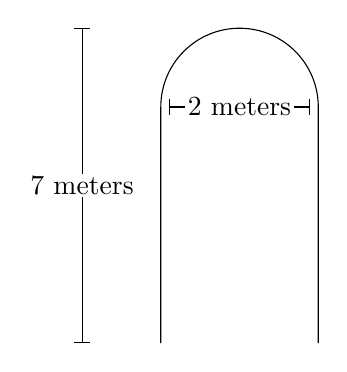
\begin{tikzpicture}
          \draw (0,0) -- (0,3) arc (180:0:1) -- (2,0);
          \draw[|-|] (-1,0) -- node[midway, inner sep=1pt, fill=white] {7 meters} (-1, 4);
          \draw[|-|] (0.1,3) --  node[midway, inner sep=1pt, fill=white] {2 meters} (1.9,3);
        \end{tikzpicture} \hspace{36pt}
        \begin{tikzpicture}
          \draw (0,0) -- (0,2) arc (180:0:2) -- (4,0);
          \draw[|-|] (-1,0) -- node[midway, inner sep=1pt, fill=white] {7 meters} (-1, 4);
          \draw[|-|] (0.1,2) --  node[midway, inner sep=1pt, fill=white] {4 meters} (3.9,2);
        \end{tikzpicture}
      \end{center}

      Now let's \hl{\textbf{write a formula}} for the height of the side wall, \hl{\textbf{defining any variables we use.}}
       \begin{center}
        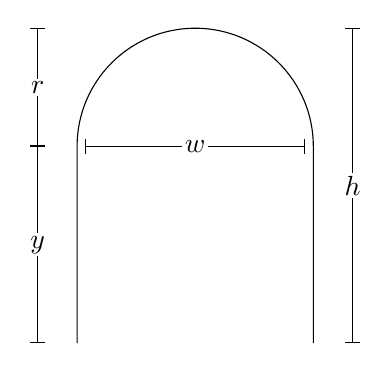
\begin{tikzpicture}
          \draw (0,0) -- (0,2.5) arc (180:0:1.5) -- (3,0);
          \draw[|-|] (-0.5,0) -- node[midway, inner sep=1pt, fill=white] {$y$} (-0.5, 2.5);
          \draw[|-|] (-0.5, 2.5) -- node[midway, inner sep=1pt, fill=white] {$r$} (-0.5, 4);
          \draw[|-|] (0.1,2.5) --  node[midway, inner sep=1pt, fill=white] {$w$} (2.9,2.5);
          \draw[|-|] (3.5,0) -- node[midway, inner sep=1pt, fill=white] {$h$} (3.5, 4);
        \end{tikzpicture}
      \end{center}
     Let's use $r$ to represent the height from the bottom of the semicircle to the top of the semicircle and $h$
     to represent the total height of the archway. Then $y=h-r$. 
     
     To write $y$ as a function of $w$, we need to \hl{\textbf{relate the variables}} using \hl{\textbf{information we know}} about the situation. We know that the
     total height of the archway is 7 meters, so $h=7$. Also, we can see that $r$ is the radius of the semicircle
     and $w$ is the diameter, which means that $r=\frac{1}{2}w$. We can substitute these expressions for $h$ and $r$
     to get $y=\boxed{7-\frac{1}{2}w}$. 
    \end{solution}

    

    

  \item
    \begin{problem}[\vfill]
      Express the area enclosed by the archway as a function of $w$.
    \end{problem}

    \begin{solution}
      \hl{\textbf{The goal}} is to write the \goal{area} enclosed by the archway as a function of the \indvar{width}
      of the archway. Using our pictures from before, we can \hl{\textbf{write a formula}} for the area:
      $A = yw + \frac{1}{2}\pi r^2$, where $yw$ is the area enclosed by the rectangle and $\frac{1}{2}\pi r^2$ is the 
      area enclosed by the semicircle.

      To write $A$ as a function of $w$, we need to \hl{\textbf{relate the variables}} we used to $w$. From part (a),
      we know that $y=7-\frac{1}{2}w$, and $r = \frac{1}{2}w$. Substituting these expressions into the formula
      for the area, we get
      $A = \boxed{(7-\tfrac{1}{2}w)w + \frac{1}{2} \pi (\tfrac{1}{2}w)^2}$.
    \end{solution}

  \item
    \begin{problem}[\vfill]
      Express the perimeter of the archway (excluding the floor) as a
      function of $y$.
    \end{problem}

    \begin{solution}
      \hl{\textbf{The goal}} is to write the \goal{perimeter} of the archway as a function of the \indvar{width}
      of the archway. Using our pictures from before, we can \hl{\textbf{write a formula}} for the perimeter:
      $P = 2y + \frac{1}{2} \pi w$, where $2y$ is the length of the two straight sides and $\frac{1}{2}\pi w$ is the 
      perimeter of the semicircle.

      To write $A$ as a function of $w$, we need to \hl{\textbf{relate the variables}} we used to $w$. From part (a),
      we know that $y=7-\frac{1}{2}w$. Substituting this expression into the formula for the perimeter, we get
      $P = \boxed{2(7-\tfrac{1}{2}w)+\frac{1}{2}\pi w}$.
    \end{solution}

  \end{enumerate}

  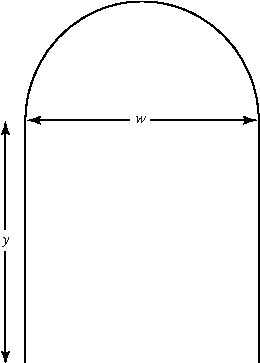
\includegraphics{art/go01p48}

  \item   % adapted from 1.3 \#30 in Robin's book

  A cistern for storing water is in the shape of a right circular cone with radius 8 feet and height 40 feet.\probonly{\footnote{Useful fact: The volume of a cone with radius $R$ and height $H$ is $\frac{1}{3}\pi R^2H$.}} (The tip is at the bottom.)

  \note{This problem introduces students to similar triangles. Students will often have trouble figuring out when to use similar triangles as opposed to Pythagorean Theorem, so have them articulate what makes two triangles similar.

    Really encourage students to explicitly write a goal, like ``Goal: Find $h(r)$.'' }

  \begin{enumerate}
  \item
    \begin{problem}[\vfill]
      Suppose the cistern is filled part-way with water. Express the height of the water as a function of the radius of the surface of the water. What's the domain of this function?
    \end{problem}
    
     \begin{solution}
      \begin{enumerate}[label=\arabic*.]
      \item \hl{\textbf{Understand the Problem.}}

        \begin{itemize}
        \item \hl{\textbf{Goal:}} Express the \goal{height} of the water as a
        function of the \indvar{radius} of the surface of the water.

          \hl{\textbf{Know:}} radius of cone = 8 feet, height of cone = 40 feet

        \item Again, drawing pictures is a good way to get a feel for the situation.

        \begin{center} 
        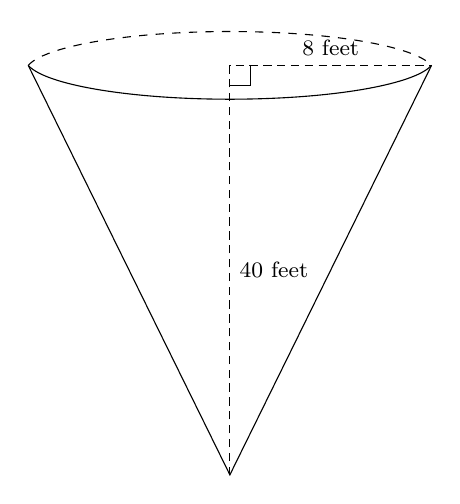
\begin{tikzpicture}[scale =1.3]
          \draw[dashed, ] (0, 0) arc (170:10:2cm and 0.4cm)coordinate[pos=0] (a);
          \draw [] (0, 0) arc (-170:-10:2cm and 0.4cm)coordinate (b);
          \draw[densely dashed, ] ([yshift=-4cm]$(a)!0.5!(b)$) -- node[right, font=\footnotesize] {$40$ feet}coordinate[pos =.95] (aa)($(a)!0.5!(b)$)
          -- node[above , font=\footnotesize] {$8$ feet}coordinate[pos=0.1] (bb) (b);
          \draw [] (aa) -| (bb);
          \draw [](a) -- ([yshift=-4cm]$(a)!0.5!(b)$) -- (b);
        \end{tikzpicture} \hspace{1cm}
        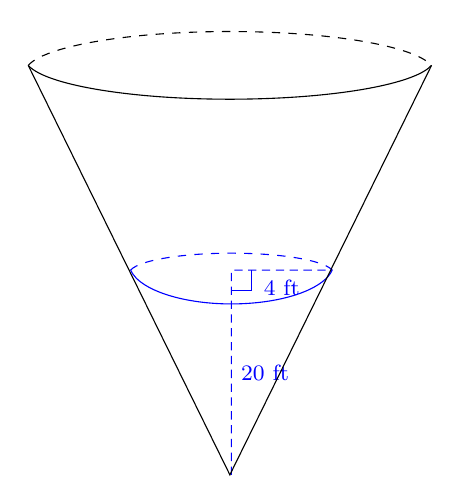
\begin{tikzpicture}[scale=1.3]
          \draw[dashed] (0, 0) arc (170:10:2cm and 0.4cm)coordinate[pos=0] (a);
          \draw[dashed, blue] (1, -2) arc (170:10:1cm and 0.2cm)coordinate[pos=0] (d) ;
          \draw [blue] (1, -2) arc (-170:-10:1cm and 0.4cm)coordinate (c);
          \draw [] (0, 0) arc (-170:-10:2cm and 0.4cm)coordinate (b);
          \draw[densely dashed, blue] ([yshift=-2cm]$(c)!0.5!(d)$) -- node[right, font=\footnotesize] {$20$ ft}coordinate[pos =.9] (dd)($(c)!0.5!(d)$)
          -- node[below, font=\footnotesize] {$4$ ft}coordinate[pos=0.2] (cc) (c);
          \draw [](a) -- ([yshift=-4cm]$(a)!0.5!(b)$) -- (b);
          \draw [blue] (dd) -| (cc);
        \end{tikzpicture}
        \end{center}
        \end{itemize}

      \item Since our goal is the \goal{height}, let's \hl{\textbf{write a
      formula}} for it, \hl{\textbf{defining any variables we use.}}
      
      Let $h$ be the height of the water and $r$ be the radius of the
      surface of the water. 
      
      \begin{center}
      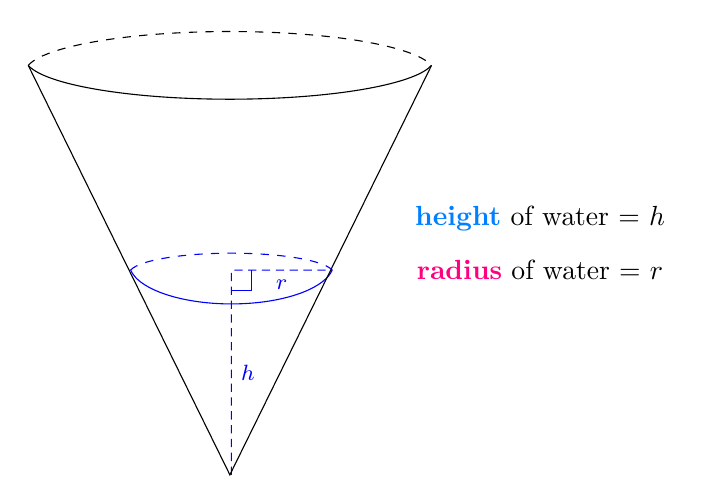
\begin{tikzpicture}[scale=1.3]
          \draw[dashed] (0, 0) arc (170:10:2cm and 0.4cm)coordinate[pos=0] (a);
          \draw[dashed, blue] (1, -2) arc (170:10:1cm and 0.2cm)coordinate[pos=0] (d) ;
          \draw [blue] (1, -2) arc (-170:-10:1cm and 0.4cm)coordinate (c);
          \draw [] (0, 0) arc (-170:-10:2cm and 0.4cm)coordinate (b);
          \draw[densely dashed, blue] ([yshift=-2cm]$(c)!0.5!(d)$) -- node[right, font=\footnotesize] {$h$}coordinate[pos =.9] (dd)($(c)!0.5!(d)$)
          -- node[below, font=\footnotesize] {$r$}coordinate[pos=0.2] (cc) (c);
          \draw [](a) -- ([yshift=-4cm]$(a)!0.5!(b)$) -- (b);
          \draw [blue] (dd) -| (cc);
          \draw (5, -1.5) node{\goal{height} of water = $h$};
          \draw (5, -2) node{\indvar{radius} of water = $r$};
        \end{tikzpicture}
        \end{center}

      To come up with a relationship between $h$ and $r$, we
      can use similar triangles.

      \begin{center}
        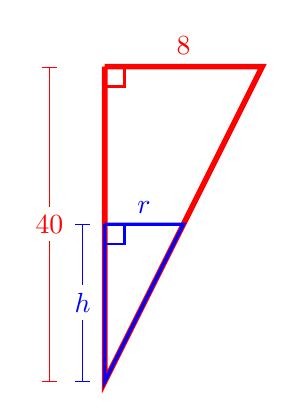
\begin{tikzpicture}
            \draw[line width=2pt, red] (0,0) -- node[above] {$8$} (2,0) -- (0,-4) -- (0,0);
            \draw[red, |-|, xshift=-20pt] (0,0) -- node[midway, fill=white, inner sep=1mm]{$40$} (0, -4);
            \draw[blue, |-|, xshift=-8pt] (0,-2) -- node[midway, fill=white, inner sep=1mm]{$h$} (0, -4);
            \draw[very thick, blue] (0,-2) -- node[above] {$r$} (1, -2) -- (0, -4) -- (0,-2);
            \draw[red, thick] (0,-0.25) -- (0.25,-0.25) -- (0.25,0);
            \draw[blue, thick] (0,-2.25) -- (0.25, -2.25) -- (0.25, -2);
        \end{tikzpicture}
      \end{center}

      The ratios of corresponding side
      lengths of similar triangles are the same, so $\frac{h}{40} =
      \frac{r}{8}$. Solving this equation for $h$, we get $h = \boxed{5r}$.

      The domain is the set of all possible inputs into our function, so the set of all possible values of $r$. 
      Since the radius of the cistern is 8, $r$ cannot be more than 8. The domain of our function is $\boxed{0 \leq r \leq 8}$.
      \end{enumerate}
    \end{solution}

  \item
    \begin{problem}[\vfill\newpage]
      Express the volume of water in the cistern as a function of the height of water in the cistern. What's the domain of this function?
    \end{problem}

    \begin{solution} 
      This is similar to the problem above, but now \hl{\textbf{our goal}} is to write the 
      \goal{volume} of the water as a function
      of the \indvar{height} of the water. Since we've already written what we know about the problem and have drawn 
      pictures, now, let's \hl{\textbf{write a formula}} for the volume. 
      
      For a cone, $V = \frac{4}{3}\pi r^2 h$, where $V$ is the volume of the cone, $r$ is the radius of the cone, and
      $h$ is the height of the cone. This formula applies to the water and not just the cistern.
      
      Now we need to \hl{\textbf{relate the variables we've used}} to write the volume in terms of only the height,
      so we need to \hl{\textbf{use something we know about the situation.}} Here we need to use the fact that $h = 5r$,
      which we came up with in part (a). Rearranging this into $r=\frac{h}{5}$ allows us to substitute $\frac{h}{5}$ for
      $r$ in our volume formula. $V(h) = \frac{1}{3} \pi ( \frac{h}{5})^2 h = \boxed{ \frac{1}{75} \pi h^3}$.

      The domain is the set of possible inputs. In this case the domain is the possible values of $h$. 
      Since the cistern is $40$ feet tall, the domain is $\boxed{0 \leq h \leq 40}$.
    \end{solution}

  \end{enumerate}

\end{enumerate}
\end{document}
